\section{Formal Model} \label{sec:model}

To articulate how \lang works, we present a core model \corelang,
modeling the essence of behavioral contracts and Solidity.
Modulo minor syntactic difference, \corelang is entirely a subset of Solidity. %\xx{this sentence is confusing} 
This section presents \corelang's abstract syntax, static and
translation semantics, which guide the actual implementation (\Cref{sec:impl}). 

\newcommand{\AddrCall}[3]{
  \K \texttt{(} {#1} \texttt{).}{#2} \texttt{(} {#3} \texttt{)}
}
\newcommand{\Call}[2]{
  {#1}\left({#2}\right)
}
\newcommand{\SpecCall}[3]{
  {#1}\texttt{(} {#2} \texttt{)}: \texttt{(}{#3}\texttt{)}
}
\newcommand{\SpecCond}[3]{
  \Keywd{requires}~ {#1} ~\Keywd{ensures}~ {#2} ~\Keywd{where}~ {#3}
}
\newcommand{\FunDef}[6]{
  {#1} ~\Keywd{fun}~ {#2}\left({#3}\right): ~ \left({#5}\right) ~ {#4}  ~\left\{~ {#6} ~\right\}
}
\newcommand{\FunType}[4]{
  \Keywd{fun}~ {#1}\texttt{(} {#2} \texttt{)}: \texttt{(} {#4} \texttt{)} ~ {#3} 
}
\newcommand{\FunTypeNR}[4]{
  \Keywd{fun}~ {#1}\texttt{(} {#2} \texttt{)} ~ {#3} 
}
\newcommand{\Contract}[3]{
  \Keywd{contract}~ {#1}~ \texttt{\{}~ {#2} \texttt{;}~ {#3} ~\texttt{\}}
}
\newcommand{\Interface}[2]{
  \Keywd{interface}~ {#1}~ \texttt{\{} ~ {#2} ~\texttt{\}}
}

\newcommand{\F}{\mathcal{F}}
\newcommand{\C}{\mathcal{C}}
\newcommand{\I}{\mathcal{I}}
\newcommand{\K}{\kappa}

\begin{figure}
\small
  \begin{alignat*}{3}
    &~ &n & \in && \mathbb{Z} \qquad b \in \mathbb{B} \qquad x,y,f,\K \in \Typ{Id}   \\
    \Typ{Data Types}  &~ t, r && :=\ && \Keywd{unit} \mid \Keywd{int} \mid \Keywd{uint} \mid \Keywd{bool} \mid \Keywd{address} \mid \dots \\
                      %&~   && \mid\ && \Keywd{mapping} ~t~ \Keywd{=>} ~t \mid \Keywd{struct} ~x~ \Keywd{\{}~ d^* ~\Keywd{\}} \\
                      % &~   && \mid\ && \FunType{f}{t^*}{m}{t^*} \\
    \Typ{Type~Decl}   &~ d && :=\ && t ~ x \hspace{3.6em}
    \Typ{Values}       ~ v :=\ n \mid b \\
    \Typ{Assignable}  &~ a && :=\ && d \mid x \hspace{3em}
    \Typ{Target}       ~ \tau :=\    f \mid \K \Keywd{(} x \Keywd{).}f \\
    %\Typ{Projection}  &~ p && :=\ && \Keywd{.}x \mid \Keywd{[}e\Keywd{]} \\
    %\Typ{Call~Opts}   &~ \ell&& :=\ && \Keywd{value} \mid \Keywd{gas} \mid \dots \\
    \Typ{Expressions} &~ e && :=\ && x \mid v \mid e ~op~ e % \mid e p^+ 
                                \mid f \texttt{(} e^* \texttt{)}
                                \mid \AddrCall{e}{f}{e^*} \\
    % \mid x \mid e p^+ \\
    \Typ{Statements}  &~ s && :=\ && d \mid e \mid s; s \mid a ~\Keywd{=}~ e \mid \Keywd{return}~ e \\ %\mid \Keywd{revert} \\
                      &~   && \mid\ && \Keywd{if (}e\Keywd{) \{}~ s ~\Keywd{\} else \{}~ s ~\Keywd{\}} \\
    \Typ{Spec}        &~ \sigma && :=\ && \SpecCall{\tau}{x^*}{y^*} \SpecCond{e}{e}{\sigma^*} \\
    \Typ{Modifiers}   &~ m && :=\ && \Keywd{public} \mid \Keywd{private} \\
    \Typ{Fun~Decl}    &~ d_f && :=\ && \FunType{f}{d^*}{m}{r^*} \\
    \Typ{Fun~Def}     &~ \F&& :=\ && \sigma ~ d_f ~ \Keywd{\{} ~ s ~ \Keywd{\}} \\
    \Typ{Contract}    &~ \C&& :=\ && \Contract{\K}{d^*}{\F^*} \\
    \Typ{Interface}   &~ \I&& :=\ && \Interface{\K}{d_f^*}
  \end{alignat*}
  % \vspace{-2em}
  \vspace{-1.5em}
  \caption{The abstract syntax of $\lambda_\lang$.}
  \label{fig:syntax}
\end{figure}
%%% Local Variables:
%%% mode: latex
%%% TeX-master: "paper"
%%% End:

\newcommand{\Edenot}[1]{\mathsf{E}\llbracket{#1}\rrbracket}
\newcommand{\Sdenot}[1]{\mathsf{S}\llbracket{#1}\rrbracket}
\newcommand{\Fdenot}[1]{\mathsf{F}\llbracket{#1}\rrbracket}

\newcommand{\Unwrap}[1]{ \textit{unwrap}(#1) }
\newcommand{\Wrap}[1]{ \textit{wrap}(#1) }
\newcommand{\Attach}[1]{ \textit{attachSpec}(#1) }
\newcommand{\Dispatch}[3]{ \textit{dispatch}^{#1}_{#2}(#3) }

\newcommand{\rulesep}{\unskip\ \vrule\ }


\begin{figure*}[ht]
\begin{subfigure}[t]{0.40\textwidth}
  \judgement{Expression Translation}{$\Edenot{\cdot}$}
  \centering
  \small
  \begin{alignat*}{2}
    && \Edenot{x} & = x \\
    && \Edenot{v} & = \Wrap{v} \\
    && \Edenot{e_1 ~op~ e_2} & = \Unwrap{\Edenot{e_1}} ~op~ \Unwrap{\Edenot{e_2}} \\
    && \Edenot{f(e, \dots)} & = f_\textit{guard}(\Edenot{e}, \dots) \\
    && \Edenot{\kappa(e_\textit{addr})\Keywd{.}f(e, \dots)} & = \Dispatch{\kappa}{f}{\Edenot{e_\textit{addr}}, \Edenot{e}, \dots}
  \end{alignat*}
\end{subfigure}
\rulesep
\begin{subfigure}[t]{0.53\textwidth}
  \judgement{Statement Translation}{$\Sdenot{\cdot}$}
  \centering
  \small
  \begin{alignat*}{2}
    && \Sdenot{t ~ x} & = t^\uparrow ~ x  \hspace{6.25em} \Sdenot{e} = \Edenot{e} \\
    && \Sdenot{t ~ x ~\Keywd{=}~ e} & = t^\uparrow ~ x ~\Keywd{=}~ \Edenot{e}  \hspace{2em} \Sdenot{x ~\Keywd{=}~ e} = x ~\Keywd{=}~ \Edenot{e} \\
    && \Sdenot{s_1 \Keywd{;}~ s_2}  & = \Sdenot{s_1} \Keywd{;}~ \Sdenot{s_2} \\
    && \Sdenot{\Keywd{return}~ e}   & = \Keywd{return}~ \Edenot{e} \\
    %&& \Sdenot{\Keywd{revert}}      & = \Keywd{revert} \\
    && \Sdenot{\Keywd{if (}e\Keywd{) \{}~ s_1 ~\Keywd{\} else \{}~ s_2 ~\Keywd{\}}} & =
      \Keywd{if (}\Edenot{e}\Keywd{) \{}~ \Sdenot{s_1}~\Keywd{\} else \{}~ \Sdenot{s_2} ~\Keywd{\}}
  \end{alignat*}
  \end{subfigure}
  \caption{The translation semantics of $\lambda_\lang$ (statements and expressions).}
  \label{fig:translation}
\end{figure*}

\begin{figure}
  \judgement{Function Translation}{$\Fdenot{\cdot}$}
  \centering
  \small
  \begin{alignat*}{2}
    %& \Fdenot{ {\color{csspec} \SpecCall{f}{x_1, \dots}{y_1, \dots} \SpecCond{e_1}{e_2}{(\sigma_1, \dots)}} ~ \FunType{f}{t_1 ~ x_1, \dots}{\Keywd{public}}{r_1, \dots} ~ \Keywd{\{} ~ s ~ \Keywd{\}} } && = \\
    %    & \hspace{1em} \FunType{f}{t_1 ~ x_1, \dots}{\Keywd{public}}{r_1, \dots} ~ \Keywd{\{}~ \Keywd{return}~ \Unwrap{ f_\textit{guard}(\Wrap{x_1}, \dots) }  ~\Keywd{\}} && \\
    %    & \hspace{1em}  \Fdenot{ {\color{csspec} \SpecCall{f}{x_1, \dots}{y_1, \dots} \SpecCond{e_1}{e_2}{(\sigma_1, \dots)}} ~ \FunType{f}{t_1 ~ x_1, \dots}{\Keywd{private}}{r_1, \dots} ~ \Keywd{\{} ~ s ~ \Keywd{\}} } && \\
    & \mathsf{F}\llbracket {\color{csspec} \SpecCall{f}{x_1, \dots}{y_1, \dots} \SpecCond{e_1}{e_2}{(\sigma_1, \dots)}} && \\
    & \hspace{0.75em} \FunType{f}{t_1 ~ x_1, \dots}{m}{r_1, \dots} ~ \Keywd{\{} ~ s ~ \Keywd{\}} \rrbracket = && \\
        & \hspace{1.25em} \FunType{f}{t_1 ~ x_1, \dots}{m}{r_1, \dots} ~ \Keywd{\{}~ && \\
        & \hspace{2.25em} \Keywd{return}~ \Unwrap{ f_\textit{guard}(\Wrap{x_1}, \dots) }  ~\Keywd{\}} && \\
        & \hspace{1.25em}
          \FunType{f_{\textit{pre}}}{t_1^\uparrow ~ x_1, \dots}{\Keywd{private}}{} ~ \Keywd{\{} ~  \Keywd{require(} \Edenot{e_1} \Keywd{)} ~ \Keywd{\}} && \\
        & \hspace{1.25em}
          \FunType{f_{\textit{post}}}{t_1^\uparrow ~ x_1, \dots, r_1^\uparrow ~ y_1, \dots}{\Keywd{private}}{} ~ \Keywd{\{} ~ \Keywd{require(} \Edenot{e_1} \Keywd{)}  ~ \Keywd{\}} && \\
        & \hspace{1.25em}
          \FunType{f_{\textit{guard}}}{t_1^\uparrow ~ x_1, \dots}{\Keywd{private}}{r_1^\uparrow, \dots} ~ \Keywd{\{} && \\
        &   \hspace{2.25em} f_\textit{pre}(x_1, ...) && \\
        &   \hspace{2.25em} \Attach{x_1, ..., \sigma_1, \dots} && \\
        &   \hspace{2.25em} (r_1^\uparrow ~ y_1, ...) = f_\textit{worker}(x_1, \dots) && \\
        &   \hspace{2.25em} \Attach{y_1, ..., \sigma_1, \dots} && \\
        &   \hspace{2.25em} f_\textit{post}(x_1, \dots, y_1, \dots) && \\
        &   \hspace{2.25em} \Keywd{return}~ (y_1, \dots) ~ \Keywd{\}} && \\
        %&   \hspace{1.25em} \Keywd{\}}  && \\
        & \hspace{1.25em}
          \FunType{f_{\textit{worker}}}{t_1^\uparrow ~ x_1, \dots}{\Keywd{private}}{r_1^\uparrow, \dots} ~ \Keywd{\{} ~ \Sdenot{s} ~ \Keywd{\}}  &&
  \end{alignat*}
  % \vspace{-2em}
  \vspace{-2mm}
  \caption{The translation semantics of $\lambda_\lang$ (functions).}
  \label{fig:fun-translation}
\end{figure}


\subsection{Syntax}

\Cref{fig:syntax} shows the abstract syntax of \corelang, modeling the essential parts of Solidity.

% \subsubsection*{\textbf{Types}}
\bfpara{Types.}
\corelang's type universe contains integers, unsigned integers, booleans, and addresses.
Aiming for minimality, we omit compound data types such as mappings and structs.
However, our presented formalization can be extended with mappings and structs as in the implementation (Section~\ref{sec:impl}).
%In \Cref{sec:impl}, we also discuss their treatment in the implementation.\xx{their treatment? do you mean how we implement them}
%A mapping type has the domain type and codomain type.
%A struct type has a name and a list of type-and-identifier declarations.

% \subsubsection*{\textbf{Top-Levels}}
\bfpara{Top-Levels.}
At the top-level, a contract $\C$ consists of field declarations and function definitions.
These fields (type-and-identifier) declarations specify storage states, which are persistent data on the blockchain.
As in other languages, a function definition consists of its name, parameters,
return types, and its body. 
To model boundaries between multiple smart contracts, a function can be either \Keywd{public} or \Keywd{private}.
A \Keywd{public} function can be called by other contracts, and \Keywd{private} functions 
can only be called within its defining contract.
In \corelang, a specification $\sigma$ is attached to every function.

Interfaces can be declared to interact with other contracts. They contain function declarations and provide expected types of arguments and return values for address calls.
% Interfaces can only contain function declarations. Interfaces are useful 
% to specify the signatures for address calls, providing expected types of 
% arguments and return values for the calls.

% \subsubsection*{\textbf{Statements and Expressions}}
\bfpara{Statements and Expressions.}
The body of functions is simply a statement. %\xx{a statement? a ``statements'' component/symbol/..?}
A statement can be a type-and-identifier declaration (uninitialized),
an expression (e.g. calling a function for its side effects), a
composition of two statements, an assignment, a \Keywd{return} statement, a \Keywd{revert} statement,
or a conditional statement.
Both type-and-identifier declarations or identifiers can be used as assignable (left-hand side of assignments).
%Since \corelang permits both mappings and structs, which can recursively refer to
%other types, projection allows use to directly access nested data structures,
%e.g. \code{x.field1[0].field2}.
A \texttt{revert} statement aborts the execution, reverting any changes made to
the blockchain state.

An expression can be an identifier, a literal value (e.g. numbers), a binary
operation, a function call, or an address call.
Address and function calls have form $\AddrCall{e_1}{f}{e_2, \dots}$,
where $e_1$ is the target callee expression that yields an address value,
$f$ is the function name defined in the interface $\kappa$,
and $e_2, \dots$ denotes the arguments.
%The call options are optional and are only used when calling functions of other contracts. 
%The function name can also be the name of a struct, or the name of a contract/interface.
%Respectively, the function call denotes a call to the struct's constructor and 
%casting to the corresponding contract/interface. 
%We use a special identifier $\K$ for the name of contracts and interfaces.

% \subsubsection*{\textbf{Specifications}}
\bfpara{Specifications.}
Specifications are attached to top-level functions.
Each specification $\sigma$ designates a target, which is either a top-level function or
a function call of an address.
When specified for addresses, an interface name is required to provide the signature
of the corresponding function.

In addition, a specification introduces bindings for arguments and return values.
As introduced in Section~\ref{sec:examples}, the pre- and post-condition are denoted in 
the \spec{requires}-clause and \spec{ensures}-clause, respectively.
%In practice not all functions need to be specified with conditions.
%In such cases, a no-op specification is expressed where the precondition and
%postcondition are simply a boolean expression \code{true}.
In the \spec{where}-clause, programmers can specify the conditions for addresses
appeared as arguments or return values, using the same syntax as 
that for top-level function specifications.
% functional
% specification. 
\iffalse
The following snippet gives a concrete example that
attaches conditions to \code{addr} for its \code{transfer} function:
\begin{lstlisting}[language=Consol]
... where { 
  IERC20(addr).transfer(amt) requires ... ensures ... 
}
\end{lstlisting}
\fi
%\yy{can we drop "recursively" since we don't allow where inside where (correct me if I am wrong)}
%When the specification is attached to an address, we allow very flexible ways
%to specify the callee. For example, if a struct argument contains an address
%value that we would like to guard:
%\begin{lstlisting}
%// x is a struct argument whose field y is an address
%... where { x.y.f requires $\mathit{precond}$ ensures $\mathit{postcond}$ }
%\end{lstlisting}
%we can use the projection syntax to specify
%the condition when address \code{x.y} is called on function \code{f}.


\subsection{Static Semantics}
\newcommand{\fun}[1]{
  \text{#1}
}

\begin{figure}[t]
  %\judgement{Specification Typing}{$\Gamma \vdash \sigma: d_f$, $\Gamma \vdash e: t$}
  \judgement{Specification Typing}{}
  %\begin{alignat*}{2}
    %\fun{param}(\SpecCall{f}{(x : y)^*}{x^*}{y^*} ...) & = 1
  %\end{alignat*}
  \small
  \infrule[a-spec]{
    \Gamma(x_\text{addr}) = \Keywd{address} \qquad
    \Gamma' = \Gamma,~
              \boldsymbol{x}_i : \boldsymbol{t}_i \qquad
    \Gamma'' = \Gamma',~
              \boldsymbol{y}_j : \boldsymbol{r}_j \\
    \Gamma' \vdash e_1 : \Keywd{bool} \qquad
    \Gamma'' \vdash e_2 : \Keywd{bool}
  }{
    \Gamma \vdash 
    \SpecCall{\K(x_\text{addr}).f}{\boldsymbol{x}_i}{\boldsymbol{y}_j}~
    \Keywd{requires}~ e_1 ~\Keywd{ensures}~ e_2 \; : \\
    \FunType{f}{\boldsymbol{t}_i ~ \boldsymbol{x}'_i}{m}{\boldsymbol{r}_j}
  }

  \infrule[f-spec]{
    \Gamma' = \Gamma,~
              \boldsymbol{x}_i : \boldsymbol{t}_i \qquad
    \Gamma'' = \Gamma',~
              \boldsymbol{y}_j : \boldsymbol{r}_j \\
    \Gamma' \vdash e_1 : \Keywd{bool} \qquad
    \Gamma'' \vdash e_2 : \Keywd{bool} \\
    \forall k,\; \Gamma'' \vdash \sigma_k : d_{f_\text{exn}} \;\textit{s.t.}~
    \fun{target}(\sigma_k) = \K(x_\text{addr}).f_\text{exn} ~\wedge~
    d_{f_\text{exn}} \in \K
     % \fun{decl}(\fun{target}(\sigma_q^\text{\tiny addr}))
    % \Gamma \vdash \fun{addr}(\sigma) : \note{type-of-call}
  }{
    \Gamma \vdash
    \SpecCall{f}{\boldsymbol{x}_i}{\boldsymbol{y}_j} ~
    \SpecCond{e_1}{e_2}{\boldsymbol{\sigma}_k} \; : \\
    \FunType{f}{\boldsymbol{t}_i ~ \boldsymbol{x}'_i}{m}{\boldsymbol{r}_j}
  }

  \infrule[c-top]{
    \Gamma' = \Gamma,~
             \fun{id}(\boldsymbol{d}_i) : \fun{type}(\boldsymbol{d}_i),~
             \fun{id}(\boldsymbol{\F}_j) : \fun{decl}(\boldsymbol{\F}_j)
             \\
    \forall j,\; \Gamma' \vdash \fun{spec}(\F_j) : \fun{decl}(\F_j)
  }{
    \Gamma \vdash \Contract{\K}{\boldsymbol{d}_i}{\boldsymbol{\F}_j}
  }
  % \vspace{-1.5em}
  \vspace{-1mm}
  \caption{Static semantics (excerpt) of \corelang specifications. Only checkings relevant to specifications are shown.}
  \label{fig:static}
\end{figure}

%%% Local Variables:
%%% mode: latex
%%% TeX-master: "paper"
%%% End:


The syntax permits arbitrary expressions to appear as pre- and
post-conditions.
However, not all possible expressions are valid executable specifications.
For example, an arithmetic expression \spec{requires x + 1} 
is meaningless if used as a condition.
The static semantics in the form of a \emph{type system} concerns when a 
specification should be considered well-formed.

The general typing judgment takes the form of $\Gamma \vdash e : t$, where
$\Gamma$ is the typing environment, $e$ is the program, and $t$ is its type
under $\Gamma$.
For our purpose, the pre- and post-condition should be of type Boolean,
and only use well-scoped variables.
Since \corelang is a subset of Solidity except for specifications, \Cref{fig:static} only shows
typing rules relevant to function and address specifications
% and omit
with
the typing for the rest of the language omitted,
which can be built atop other existing works \cite{DBLP:conf/sp/JiaoK0S0020, Sergey2021, DBLP:conf/esorics/BartolettiGM19, DBLP:conf/fc/CrafaPZ19}.


The specification typing judgment takes the form of $\Gamma \vdash \sigma : d_f$, where $\Gamma$ is the typing environment, $\sigma$ is the specification, and $d_f$ is the declaration of the target function. The \textsc{c-top} rule examines contract well-formedness by checking if the specification 
attached to each function is well-typed. 
%\xx{what is containing function. check if the spec annotated on a function is well-typed?}
The \textsc{f-spec} rule checks if the annotated specification matches the actual function
declaration. It also checks if pre-conditions, post-conditions, and address specifications
are well-typed.
Similarly,
% The \textsc{a-spec} is similar, which 
\textsc{a-spec} checks address specifications against
the callee function defined in the declared interface.

%dynamic semantics
%\yy{do we want to model the context of contracts? (instead of reasoning one contract)}

\subsection{Translation Semantics} \label{sec:translation}


\Cref{fig:translation} defines the semantics of specifications by transforming 
specification-annotated programs to ordinary programs. 
This process orchestrates and inserts assertions when appropriate.
We use syntax-directed translation functions $\Fdenot{\cdot}$, $\Sdenot{\cdot}$,
$\Edenot{\cdot}$ to define the translation of functions, statements, and expressions, respectively.

%\note{GW: what if in the condition, user calls a guarded function? We need to translate pre/post conditions too}

% \subsubsection*{\textbf{Translating Types}}
\bfpara{Translating Types.}
One of \lang's key goals is to provide persistent monitoring of addresses.
To realize this, the translation uses a new type and value 
representation for a \emph{guarded address}, so that (1) specification
provenance is always kept along with the original address within the current contract,
and (2) operations on the original address preserve their results.

Given an ordinary type $t$ from untranslated programs, we use $t^\uparrow$
to denote its translated type. 
For example, $\texttt{address}$ is the naked type, and $\texttt{address}^\uparrow$
is the address type that can be attached with specifications. %\xx{is address a type name or varname? confusing}
For primitive types other than \texttt{address}, $t^\uparrow$ can be equal to $t$.
For compound data types such as arrays, $t^\uparrow$ should be recursively defined 
(the formalization has not modeled compound data types but we see no technical difficulty in doing so).
Moreover, a pair of runtime functions $\Wrap{}$
and $\Unwrap{}$ is used to convert between values of type $t$ and $t^\uparrow$,
satisfying the following conditions:
\begin{align*}
\Gamma \vdash e : t & \Leftrightarrow  \Gamma \vdash \Wrap{e} : t^\uparrow \\
\Gamma \vdash e : t^\uparrow & \Leftrightarrow  \Gamma \vdash \Unwrap{e} : t \\
\mathit{unwrap} & \circ \mathit{wrap} = \mathit{id} 
\end{align*}
The conversions are useful when (1) performing primitive operations, and (2)
at the boundary between \lang's monitored world and the external wild world.

At this moment, we intentionally keep the notion $t^\uparrow$ abstract, 
i.e., not giving its concrete definition, since multiple representations with their 
wrap/unwrap function could work.
A naive way to represent a guarded address is to use a \code{struct} that stores
the original address and the \emph{encoding} of the attached specifications.
However, this scheme introduces additional storage overhead.
In \Cref{sec:impl}, we discuss the implementations and optimizations that do not
introduce storage overhead for practical scenarios.
Since the address type is pervasively used in the program, our approach
uses a whole-program translation.

%\lang transform \Keywd{address} type to a struct
%type with an additional type $\mathcal{G}$ that carries the pre-/postcondition.
%At runtime when the underlying address is called,
%corresponding checks can be performed by examining this value of type $\mathcal{G}$.
%$$ \Keywd{address} \leadsto \Keywd{address} \times \mathcal{G} $$

% \subsubsection*{\textbf{Translating Functions}}
\bfpara{Translating Functions.}
To translate an annotated function $f$, \lang generates an interposition layer
that orchestrates runtime checks (\Cref{fig:fun-translation}).
The main job is performed in $f_\textit{guard}$,
which checks pre- and post-conditions, attaches specifications (from the \spec{where}-clause)
to address values, and invokes the actual function $f_\textit{worker}$,
whose body is recursively translated.
We also rewrite call-sites so that $f_\textit{guard}$ is invoked.
$f_{pre}$ and $f_{post}$ enforces the pre- and post-conditions 
respectively and aborts the call if a condition is violated.

% \begin{figure}[t]
	\centering
	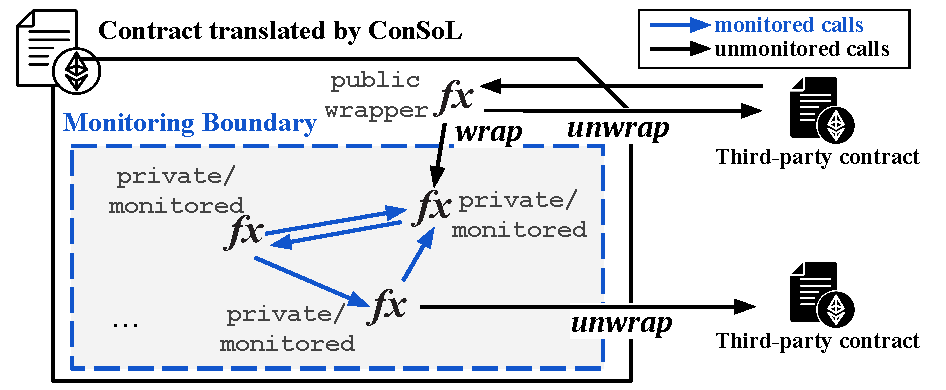
\includegraphics[width=0.85\linewidth]{monitoring_boundary.pdf}
	\vspace{-1mm}
	\caption{Monitoring boundary of guarded address calls.}
	\label{fig:monitor_bound}
	% \vspace{-1em}
\end{figure}

Additionally, a function $f$ with the same name and interface as the original function
is generated. This is used only for external calls (if the $f$ is public), which
does not observe our translated value representation for addresses.

The attachment of specifications to addresses is performed by $\mathit{attachSpec}$ 
at run-time, whose implementation depends on the representation of guarded addresses.

% \subsubsection*{\textbf{Translating Statements and Expressions}}
\bfpara{Translating Statements and Expressions.}
\lang translates statements and expressions in a recursive fashion (\Cref{fig:translation}). 
Most cases of statement translation are straightforward; they
recursively apply the translation to subcomponents.
Declared types $t$ are lifted to $t^\uparrow$
% , so that they can 
to
carry specifications.

For binary operations, we first recursively translate the operands, 
and apply $\mathit{unwrap}$ to the operands at run-time.
Since the attachment of specifications to address values may change the underlying
representing values, this is necessary to ensure our translation preserves the 
results of these operations. For example, consider the same address value $x$
attached with two different specifications $x_1$ and $x_2$. The programmer
should expect $x_1 == x_2$, which only holds after unwrapping.
In general, $\mathit{unwrap}$ should be applied when performing computation 
other than method calls over values.

Direct function calls are replaced with their guarded counterparts $f_\textit{guard}$ with arguments being translated recursively.
Address calls $\kappa(e_\mathit{addr}).f$ are replaced with calls to $\mathit{dispatch}^\kappa_f$, %\xx{grammar}
which takes the address value $e_\mathit{addr}$ in addition to the ordinary arguments as arguments.
The $\mathit{dispatch}$ inspects the specification provenance carried along with
the underlying address value, performs the corresponding checks before and after
the address calls.

% \subsubsection*{\textbf{Runtime Facilities}}
\bfpara{Runtime Facilities.}
Our translation works against a set of runtime functions, including
$\mathit{wrap}$ and $\mathit{unwrap}$ that convert value representations,
$\mathit{attachSpec}$ that bakes specification provenance into the underlying guarded address values, and
$\mathit{dispatch}$ that decodes specification provenance and performs corresponding
checked address calls. %\xx{checked calls?} 
Since $\mathit{dispath}$ makes address calls to external contract instances,
it applies $\mathit{unwrap}$ to arguments before interacting with worlds outside \lang's monitoring boundary.
Note that $\mathit{dispatch}$ is a family of functions that are specialized over the callee 
function $f$ and its interface $\kappa$.
In \Cref{sec:impl}, we describe the implementation of $\mathit{attachSpec}$ and $\mathit{dispatch}$.

% \subsubsection*{\textbf{A Concrete Example}}
\iffalse
Take the deposit function from \Cref{sec:examples-higher-order} as an example. The translated Solidity program is as follows.
\begin{lstlisting}[language=Consol]
deposit(token, amount) requires msg.sender == owner
where {
  IERC20(token).transferFrom(sender, addr, amount) returns (success)
  requires amount > 0   ensures success
}
\end{lstlisting}
\vspace{-0.25em}
\begin{lstlisting}
function deposit(address$^\uparrow$ token, uint amount) public {
  IERC20(token).transferFrom(...); // the call is now guarded
}
\end{lstlisting}
\fi

%\bfpara{A Concrete Example}
%\note{Yeah}\xx{???}

\subsection{Correctness} \label{sec:correctness}


Our translation preserves the semantics of the original program, in 
the sense that if the \lang-translated program does not raise \lang-related 
errors, then we observe the same result and state on the original program.

Moreover, \corelang guarantees that any violation will be detected 
(thus the execution will be reverted) \emph{within the 
boundary of the current contract}. 
\Cref{fig:monitor_bound} demonstrates the monitoring boundary of \corelang with the blue dashed scope.
It is straightforward to see invocations of top-level functions are redirected to
their guarded version, thus correctly monitored.
Therefore, our analysis focuses on on guarded addresses. % i.e., \textit{chainlink} in \Cref{fig:sturbyIntro}\xx{i.e., xxx in figure}\yy{added}\wac{No explanation of this spec on \textit{chainline} before this point}.
Once an address is attached with guards, there are three possible ways to unwrap it in
our translation: 
(1) the address value is used in primitive operations (e.g. comparing equality),
(2) the address value is returned to other contract instances via a public function 
(\Cref{fig:fun-translation}),
(3) the address value is passed as an argument (thus unwrapped by $\mathit{dispatch}$)
to other contract instances.
We say addresses in (2) and (3) escape our monitoring boundary, as demonstrated in \Cref{fig:monitor_bound}.
All other calls of guarded addresses stay in our boundary for effective monitoring. \looseness=-1

\begin{figure}[t]
	\centering
	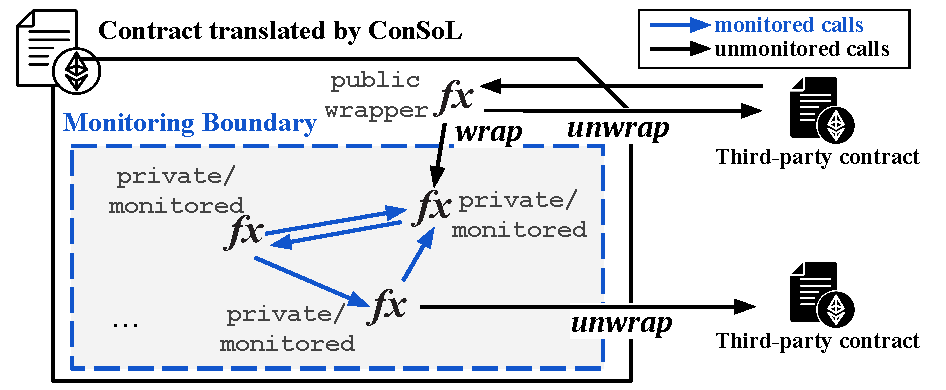
\includegraphics[width=0.85\linewidth]{monitoring_boundary.pdf}
	\vspace{-1mm}
	\caption{Monitoring boundary of guarded address calls.}
	\label{fig:monitor_bound}
	% \vspace{-1em}
\end{figure}

\renewcommand{\arraystretch}{0.8}

\begin{table}[t]
\centering
\caption{Summary of studied cases. \textit{LR} denotes LoC Reduced.}
\vspace{-1mm}
% \textit{Loss} denotes the monetary loss measured in US Dollars, and \textit{LR} denotes the percentage of lines from the assertion-based patched functions that have been translated into \lang annotations, in comparison to their original total lines.}
\small
\setlength{\tabcolsep}{2.5pt}
\label{tab:case}
\begin{tabular}{lcrlc}
\toprule
\multicolumn{1}{c}{\textbf{Project}} & \textbf{Date}     & \multicolumn{1}{c}{\textbf{Loss} (\$)} & \multicolumn{1}{c}{\textbf{Attack Type}} & \multicolumn{1}{c}{\textbf{LR}  (\%)} \\
\midrule
Umbrella~\cite{unbrellaHack}                    & 03-20-22 & 700K                     & Integer Over/Underflow                & 33.33                           \\
EFLeverVault~\cite{eflevervaultHack}                & 10-14-22 & 1M                       & Business Logic Flaw    & 25.00                           \\
N00d~\cite{n00dHack}                        & 10-26-22 & 29K                      & Reentrancy                      & 11.11                           \\
Dexible~\cite{dexibleHack}                     & 02-17-23 & 1.5M                     & Arbitrary External Call         & 11.76                           \\
SushiSwap~\cite{sushiSwapHack}                   & 04-09-23 & 3.3M                     & Unchecked User Input            & 54.55                           \\
SwaposV2~\cite{swaposv2Hack}                    & 04-16-23 & 468K                     & Erroneous Accounting            & 25.00                           \\
Unknown~\cite{unknownHack}               & 05-31-23 & 111K                     & Missing Slippage Check          & 30.00                           \\
Sturdy~\cite{sturbyHack}                      & 06-12-23 & 800K                     & Readonly Reentrancy            & 57.14                           \\
LEVUSDC~\cite{levusdcHack}                     & 06-15-23 & 105K                     & Access Control                  & 33.33                           \\
Bao~\cite{baoHack}                & 07-04-23 & 46K                      & Inflation Manipulate            & 83.33    \\
\bottomrule
\end{tabular}
\end{table}

It is worth noting that the user-provided condition expressions are also translated (\Cref{fig:fun-translation}).
This is deliberated to provide stricter semantics (known as the
``picky'' contract semantics \cite{DBLP:journals/jfp/BlumeM06}) to allow 
using guarded addresses to define conditions, which can capture more potential violations.

%translated by \lang passes all the runtime checks, 
%then the original \corelang program won't breach the attached specifications 
%when run in an identical state. \note{revisit}
% \yy{added}\note{correctness: if [p] does not have \lang-errors, then p runs without errors too.}
